\documentclass[a4paper,usenatbib]{aspdoc}
\usepackage{newtxtext,newtxmath}
\usepackage{ae,aecompl}
\usepackage{graphicx}	% Including figure files
\usepackage{amsmath}	% Advanced maths commands
\usepackage{amssymb}	% Extra maths symbols
\usepackage{lipsum}
\usepackage{float}
\usepackage{multirow}
\usepackage{booktabs}
\usepackage{geometry}
\geometry{left=25mm,right=25mm,top=25mm,bottom=25mm}

%\usepackage{cleveref}
\usepackage{siunitx}

\newcounter{simplecount}
\setcounter{simplecount}{0}
\renewcommand{\theequation}{\arabic{simplecount}}
\newcommand{\owncount}{\refstepcounter{simplecount}}

% Title
\title[]{ELE: Eigenschaften des Elektrons}

% The list of authors
\author[]{
    Riedel Lisa, Wegmann Peter
    \newauthor
    \,Gruppe 6
}

% Don't change these lines
\begin{document}
    \label{firstpage}
    \pagerange{\pageref{firstpage}--\pageref{lastpage}}
    \maketitle
  
    
    % Body
    \section{Einleitung} 
          In diesem Versuch werden zwei Experimente durchgeführt. Bei diesen handelt es sich um ein Experiment mit einer Fadenstrahlröhre, mit der die spezifische Elektronenladung berechnet wird. Bei dem zweiten Experiment handelt es sich um den Milikanversuch. Dabei wurde anstelle der Schwebemethode (Kapitel \ref{subsubsec:schweb}) die Gleichfeldmethode (Kapitel \ref{subsubsec:gleich}) verwendet. Des weiteren lässt sich aus den Ergebnissen beider Experimente die Elektronenmasse bestimmen.
        
        \noindent Im folgenden werden Vorüberlegungen zum ersten Experiment aufgestellt und anschließend konkret beantwortet.
  
            \subsection{Vorüberlegung 1}
                Wie in der Anleitung angemerkt, wurden alle Berechnung ohne Betrachtung von relativistischen Effekten durchgeführt. Die nicht relativistische Geschwindigkeit des Elektrons wird mit Hilfe der Gleichung \ref{eq:ve} ermittelt. Dabei wurde die Beschleunigungsspannung auf ihren im Versuch verwendeten Maximalwert von  $ (-)300$ V gesetzt. Setzt man diese ins Verhältnis zur Lichtgeschwindigkeit, beträgt die Elektronengeschwindigkeit $\sim 0,0343c$. Das sind ca. 3,43\%. Damit wird die im Skript genannte Faustregel erfüllt, und es darf ohne Bedenken nicht relativistisch gerechnet werden, da die relativistischen Effekte in dieser Größenordnung noch nicht relevant sind.\\          
               
            \subsection{Vorüberlegung 2}
                Es soll die Höchsttemperatur eines aus der Glühkatode emittierten Elektrons berechnet werden. Die Anfangsgeschwindigkeit sollte kleiner als 1\% der Endgeschwindigkeit bei einer Beschleunigungsspannung U = 100V sein. Hierfür wird die mittlere kinetische Energie von Molekülen verwendet, die nur 3 Freiheitsgrade besitzen. Die Gleichnungen \ref{eq:ve} und \ref{eq:ke} werden gleichgesetzt, so dass die Temperatur folgendermaßen berechnet werden kann.  \\
                \\
                    $\frac{1}{2} m v^2 = E_T \Leftrightarrow T = \frac{2}{3 k_B} q = 77,29$ K\\
                \\
                Hierbei ist $E_T$ in Gleichung \ref{eq:ke} definiert.
                Die normale Temperatur der Glühkatode entspricht etwa 1000 °C. Das ist im Verhältnis zum ermittelten Ergebnis vernachlässigbar klein. Das bedeutet, um ein Elektron auf nur 1\% seiner Endgeschwindigkeit zu bringen, müsste die Glühkathode eine Temperatur haben, die sie niemals erreichen könnte. Mit diesem Wissen kann man also zu der Näherung kommen, dass die Elektronen sich am Anfang der Beschleunigung in Ruhe befinden. Die Näherung, dass die Teilchen aus der Ruhe beschleunigt werden, ist damit berechtigt.
                
                
    
    \section{Verwendete Methoden}
        Zum Bestimmen der kinetischen Energie von Elektronen kann die folgende Formel verwendet werden. Wie in Vorüberlegung 1 aufgeführt muss die Geschwindigkeit nicht relativistisch betrachtet werden.\\
        \begin{equation}
            \owncount
            v = \sqrt{2 \cdot \frac{q}{m} \cdot U_B}
            \label{eq:ve}
        \end{equation}\\
        Mit $v$ als Geschwindigkeit, $q$ als Ladung, $m$ als Masse und $U_B$ als Beschleunigungsspannung.\\
        Die mittlere kinetische Energie von Molekülen mit 3 Freiheitsgrade kann folgendermaßen gewonnen werden:
        \begin{equation}
            \owncount
            E_T = \frac{3}{2}k_B T
            \label{eq:ke}
        \end{equation}\\
        Mit $T$ als der Temperatur in Kelvin und der Boltzmannkonstante $k_B = 1,38 \cdot 10^{-23}$.
    

        \subsection{Spezifische Elektronenladung}\label{subsec:spec}
            Für die Berechnung der spezifischen Elektronenladung muss zuerst das Magnetfeld der Helmholtzspule, in der das Experiment stattfindet, berechnet werden. Der Vorteil einer solchen Spule ist, dass sie aus zwei, parallel zueinanderstehenden Leiterschleifen besteht. Dieses Konstrukt ermöglicht es ein fast nahezu homogenes Magnetfeld im Bereich zwischen den Schleifen zu schaffen. Die magnetische Induktion für diesen Versuch relevanten Bereich lässt sich dann wie folgt beschreiben. \\
            \begin{equation}
                \owncount
                B = \mu_0 \left(\frac{4}{5}\right)^\frac{3}{2}N\frac{I}{R}
            \end{equation}\\
            Die Anzahl der Spulenwindungen ist N und der Radius der Spule ist R. Beide Größen sind in der Anleitung mit Unsicherheit angegeben.\\
            Für die Ermittlung der spezifischen Elektronenladung in einem Magnetfeld werden die wirkenden Kräfte gleichgesetzt. Dies sind die Beträge der Lorentzkraft und der Normalkraft, die auf das Teilchen in der Bahnkurve wirken. In dieser Beziehung gehen die angelegte Spannung $U_B$ und der Radius der Kreisbahn $r_K$ mit ein.\\
            \begin{equation}
                \owncount
                \frac{q}{m} = \frac{2U_B}{B^2r_K^2}
                \label{eq:sl}
            \end{equation}\\
        
        \subsection{Milikanversuch}\label{subsec:milikan}
            Für die spätere Berechnung der Elektronenmasse, muss die Elementarladung $e$ des Elektrons berechnet werden. Wie in der Anleitung (\cite{anleitung}) beschrieben, kann diese unter anderem durch Messungen der Geschwindigkeiten von Öltröpfchen in einem Kondensator berechnet werden. Dabei bieten sich zwei unterschiedliche Methoden an.  
            
            \subsubsection{Schwebemethode}\label{subsubsec:schweb}
                Bei dieser Methode handelt es sich für den praktischen Gebrauch zu umständliche Methode, weshalb diese nicht verwendet wurde. Bei der Schwebemethode wird versucht, die Tröpfchen ins schweben zu bringen. Ist der Gleichgewichtszustand erreicht, so wird das elektrische Feld ausgeschaltet. Anschließend lässt sich sowohl Tröpfchenradius $r_0$ als auch dessen Ladung $q$ durch Formel 21 und Formel 22 (siehe \cite{anleitung}) berechnen. Hierbei ist eine sehr exakte Einstellung des elektrischen Feldes von Nöten, was jedoch nur schwer möglich ist.     
            
            \subsubsection{Gleichfeldmethode}\label{subsubsec:gleich}
                Die in diesem Versuch bevorzugte Methode verzichtet auf eine exakte Einstellung des elektrischen Feldes, und fokussiert sich auf die Messung der Steigzeit $t_{\mathrm{steig}}$ und Sinkzeit $t_{\mathrm{sink}}$. Somit kann die Einstellung des elektrischen Feldes zwischen den Kondensatorplatten frei gewählt werden. Wurden $t_{\mathrm{steig}}$ und $t_{\mathrm{sink}}$ gemessen, sowie die verwendete elektrische Feldstärke $U$ vermerkt, so lässt sich $r_0$ und $q$ durch folgende Formel berechnen.
                \begin{equation}
                    \owncount
                    r_{0}=\frac{3}{2} \sqrt{\frac{\eta_{\mathrm{Luft}}\left(v_{\mathrm{steig}}+v_{\mathrm{sink}}\right)}{\rho_{\Delta} \cdot g}}
                    \label{eq:radius}
                \end{equation}
                \begin{equation}
                    \owncount
                    q=\frac{3 \pi \cdot d}{U} \cdot \eta_{\mathrm{Luft}} \cdot r_{0} \cdot\left(v_{\mathrm{steig}}-v_{\mathrm{sink}}\right)
                    \label{eq:charge}
                \end{equation}
                Bei $\eta_{\mathrm{Luft}}$ handelt es sich um die Viskosität der Luft und $\rho_{\Delta} := \rho_{\mathrm{Oel}} - \rho_{\mathrm{Luft}}$ um die effektive Dichte.
                
                \noindent Da die einfache Verwendung der Stokeschen-Reibungskraft auf den in Kapitel \ref{subsec:resmilikan} gemessenen Radien zu Ungenauigkeiten führt, muss für $\eta_{\mathrm{Luft}}$ die Cunningham-Korrektur unternommen werden.
                \begin{equation}
                \owncount
                    \eta_{\mathrm{korr}}=\eta_{\mathrm{Luft}} \cdot\left(1+A \cdot \frac{\lambda}{r_{0}}\right)^{-1}
                \end{equation}
                Für die korrigierten Formel für $r_{\mathrm{korr}}$ und $q$ siehe Formel 29 und Formel 39 in der Anleitung (\cite{anleitung}).
                
        
        \subsection{Masse des Elektrons}
            Durch Kombination der Ergebnisse von Kapitel \ref{subsec:spec} und Kapitel \ref{subsec:milikan} ist es, wie in Kapitel \ref{subsec:emass} gezeigt, möglich, die Elektronenmasse zu berechnen.
            Dabei wird Formel \ref{eq:sl} verwendet.
            \begin{equation}
            \owncount
                \frac{q}{m} = \frac{-e}{m} = e_{\mathrm{spezifisch}} \Leftrightarrow m = \frac{-e}{e_{\mathrm{spezifisch}}}
                \label{eq:slmass}
            \end{equation}
            Bei $e_{\mathrm{spezifisch}}$ handelt es sich um die spezifische Elektronenladung, bei $e$ um die Elementarladung des Elektrons, welche in Kapitel \ref{subsec:specelectron} und Kapitel \ref{subsec:resmilikan} berechnet werden.
    
    
    \section{Experimentelles Vorgehen}
        \subsection{Spezifische Elektronenladung}
            Das Experiment zur Bestimmung der spezifischen Elektronenladung ist folgendermaßen aufgebaut. In einem Neongas befülltem Glaskolben befindet sich das Fadenstrahlrohr mit Elektronenkanone. Diese Kanone besteht aus einer Heizspirale, einer Kathode und einer Lochanode und ist an ein Hochspannungsgerät angeschlossen. Der Glaskolben befindet sich in einer Helmholtzspule, mit der ein homogenes Magnetfeld erzeugt wird. Durch das Neongas ist es möglich die Elektronen, die aus der Kathode austreten und dann zur Anode beschleunigt werden, sichtbar zu machen. Sie stoßen dabei mit den Gasteilchen zusammen, und bilden einen Leuchtstrahl. Das erzeugt Magnetfeld lenkt sie dann auf eine Kreisbahn. Diese entsteht, da die Lorentzkraft senkrecht auf der Bewegungsrichtung des Elektronenstrahls wirkt und senkrecht auf das Magnetfeld steht.\\
            Es wurden zwei Messreihen aufgenommen. Bei beiden Messreihe sollte ein Radius von $30$, $40$ und $50$ mm eingestellt werden. Bei der ersten Messreihe sollte der Strom auf die Spule konstant auf $1,3$ A gehalten werden und der Radius mithilfe des Spannungsreglers eingestellt werden. Hierfür wurde die Beschleunigungsspannung passend eingestellt und mit der Wehneltspannung nachjustiert. Zu beachten war, dass die Wehneltspannung nicht mehr als $10$ V betragen durfte, da das Gerät sonst beschädigt werden könnte.\\
            Bei der zweiten Messreihe wurde die Beschleunigungsspannung auf $U_B = 125$ V eingestellt. Die Einstellung des Radius erfolgte mit dem angelegten Strom auf die Spule.\\
            Bei beiden Messreihen wurden die Spannung und der Strom mit einem digitalen Multimeter abgelesen. Jede Messreihe wurde für jeden Radius 10mal wiederholt. Das Ablesen des Radius erfolgte mit einer Skala innerhalb des Glaskolbens. Aufgrund eines Ablesefehlers, werden in den Messreihen die Radien $25$, $30$ und $35$ mm betrachtet.\\ 
        
        \subsection{Milikanversuch}
            Bei dem Versuchsaufbau des Milikanversuchs handelt es sich um einen waagrechten Plattenkondensator (Plattenabstand d = (6,00 $\pm$ 0,05) mm mit angeschlossenen, verstellbaren Hochspannungsregler mit ganzzahliger Spannungsanzeige. An dem Plattenkondensator befindet sich zusätzlich eine kleine Öffnung, durch welche feine Öltröpfchen in den Kondensator eingesprüht werden können. Durch einer weiteren Öffnung können die eingesprühten Öltröpfchen durch ein verschiebbares Messmikroskop mit Mikrometerokular beobachtet werden, an welchem sich eine Kamera befindet. In der verwendeten Kamerasoftware wurde für die Messung von $t_{\mathrm{steig}}$ und $t_{\mathrm{fall}}$ ein Liniengitter aktiviert. Für das Steigen oder Fallen der Öltröpfchen kann das elektrische Feld umgepolt werden. Der Abstand zwischen den Linien liegt bei einem gemessenen Wert von $d_{\mathrm{Linien}} = 1,8$ mm.
            
            \noindent Es wurden 20 Messungen verschiedener Öltröpchen durchgeführt. Dabei wurde bei jeder Messung sowohl $t_{\mathrm{steig}}$ und $t_{\mathrm{fall}}$, als auch die jeweilig eingestellte Feldstärke $U$ aufgezeichnet. Die Zeitmessungen werden anschließend verwendet um die Steig- und Fallgeschwindigkeit $v_{\mathrm{steig}}$ und $v_{\mathrm{fall}}$ zu berechnen.
            
            \noindent Aufgrund der wenigen Messungen verwenden die Ergebnisse in Kapitel \ref{sec:result} jeweils 20 weitere Messungen von zwei weiteren Gruppen und 22 Messungen der Versuchsleitung. 
            
            \subsubsection{Verwendete Einstellungen}
                Aufgrund der Temperatur- und Druckabhängigkeit von Formel \ref{eq:radius} und Formel \ref{eq:charge} sind eine Temperatur- und Druckmessung des Labors von Nöten. Hierbei wurde $T = 23$ °C und ein Druck $p = 956,8$ mbar gemessen. Dementsprechend wurde $\rho_{\mathrm{Oel}} = 871 \frac{\mathrm{kg}}{\mathrm{m^3}}$ gewählt. Weitere wichtige Konstanten, die für die in Kapitel \ref{sec:result} erzielten Ergebnisse verwendet wurden, sind in Tabelle \ref{tab:config} dargestellt.
                
                \begin{table}
                    \centering
                    \begin{tabular}{c|cccc}
                        \multicolumn{1}{c}{Datensatz} & \multicolumn{4}{c}{Konstanten} \\
                        \cmidrule(l){0-0}\cmidrule(lr){2-5}
                        \toprule
                         & $d_{\mathrm{Linien}}$ [mm]    & $T$ [°C]   & $\rho_{\mathrm{Luft}}$ [mbar]  & $\eta_{\mathrm{Luft}}$ [$\mu$Pa $\cdot$ s] \\ 
                            1   & 1,8     & 23,0        & 1,12     & 17,1\\ 
                            2   & 2,2     & 23,5        & 1,12     & 17,1 \\ 
                            3   & 1,9     & 23,1        & 1,12     & 17,1 \\ 
                            4   & $\sim$2,0    & 23,0   & 1,12  & 17,1  \\
                        \bottomrule
                    \end{tabular}
                    \caption{Verwendete Konstanten um $r_0$ und $q$ durch Formel \ref{eq:radius} und Formel \ref{eq:charge} zu berechnen. Bei Datensatz 4 hatte jede der 22 Messungen einen unterschiedlichen Linienabstand $d_{\mathrm{Linien}}$.}
                    \label{tab:config}
                \end{table}
    
    
    \section{Ergebnisse}\label{sec:result}
        In diesem Kapitel werden die gesamten Ergebnisse beider Experimente dargestellt und kurz diskutiert. In Kapitel \ref{subsec:emass} findet sich, durch Kombination beider Experimente, die Berechnung der Masse des Elektrons\footnote{Der Sourcecode zur Berechnung von $q$ und $r_0$ findet sich unter \url{https://github.com/Wegii/AP2-SS19}\label{note:source}}.

        \subsection{Spezifische Elektronenladung}\label{subsec:specelectron}
            Aus den beiden Messreihen konnten zu jedem Radius die Mittelwerte mit Unsicherheit der spezifischen Elektronenladung gewonnen werden, die in Tabelle \ref{tab:sel} dargestellt sind. 
            \begin{table}
                \centering
                \begin{tabular}{c|c|c}
                    \multicolumn{1}{c}{ Radius p [mm]} & \multicolumn{1}{c}{$I = 1,3$ A = const} & \multicolumn{1}{c}{$U_B = 125$ V = const}\\
                    \cmidrule(l){0-0}\cmidrule(lr){2-2}\cmidrule(lr){3-3}
                    \toprule
                    25 & $(1,84 \pm 0,85) \cdot 10^{11} \frac{C}{Kg}$ & $(1,67 \pm 0,51) \cdot 10^{11} \frac{C}{Kg}$ \\
                    30 & $(1,72 \pm 0,71) \cdot 10^{11} \frac{C}{Kg}$ & $(1,72 \pm 0,45) \cdot 10^{11} \frac{C}{Kg}$ \\
                    35 & $(1,69 \pm 0,66) \cdot 10^{11} \frac{C}{Kg}$ & $(1,75 \pm 0,41) \cdot 10^{11} \frac{C}{Kg}$ \\
                    \bottomrule
                \end{tabular}
                \caption{Messwerte mit Unsicherheiten der spezifischen Elektronenladung}
                \label{tab:sel}
            \end{table}
            \\
            Aus diesen Ergebnissen kann dann das Gesamtergebnis, mit Hilfe des gewichteten Mittelwerts, ermittelt werden. 
            \begin{center}
                $\mathbf{\frac{e}{m} = -(1,72 \pm 0,05) \cdot 10^{11} \frac{C}{kg}}$
            \end{center} 
            Dies kommt dem Literaturwert von $\frac{e}{m} = -1,75 \cdot 10^{11} \frac{\mathrm{C}}{\mathrm{kg}}$ nahe (\cite{gerthsen}).
            Für die \textbf{statistische} Unsicherheit wurde für jeden Radius der Mittelwert aus der variierenden Spannung oder dem variierenden Strom ermittelt. Danach wurden die statistische Unsicherheit und der Mittelwert der statistischen Unsicherheit berechnet. Da die Messreihe nur 10 Messergebnisse lang war, wurde eine Korrektur der wenigen Messergebnisse mit Hilfe der Student-t-Verteilung vorgenommen. Das Vertrauensniveau beträgt 68,2\%. Die Unsicherheiten wurden dann partiell fortgepflanzt.\\
            Um die \textbf{systematische} Unsicherheit zu ermitteln wurden folgende Annahmen getroffen.\\
            Bei der Verwendung von Multimeter sollte bei der Angabe von Unsicherheiten immer im Datenblatt des jeweiligen Gerätes nachgesehen werden, da diese vom Hersteller abhängig sind. Dies wurde von uns nicht beachtet, weshalb geschätzt wurde. Das ist eine weitere Unsicherheit, die bei den systematischen Unsicherheiten mit einfließen sollte. 
            Bei der Messreihe mit konstantem Strom, der über ein digitales Multimeter angezeigt worden ist, wurde mit einer Unsicherheit von $0,1$ A gerechnet.\\
            Bei der Messreihe mit konstanter Spannung, die ebenfalls mit einem digitalen Multimeter abgelesen wurde,  wurde die Unsicherheit nach einer Faustregel geschätzt. Diese besagt, die Unsicherheit beträgt in etwa 3\% der gemessenen Spannung. Für die verwendete Spannung von $U_B = 125$ V beträgt das eine Unsicherheit von $\sim 3,75$ V. \\
            Die Unsicherheit der Messmarkierung wurde mit $3$ mm angenommen. Dabei sind sowohl die Unsicherheit des Bahndurchmessers als auch die Dicke des Bahnradius miteinbezogen. 
          
        \subsection{Milikanversuch}\label{subsec:resmilikan}
            Aus den aufgenommenen Datenpunkte ist es nun durch Betrachtung der Ladungsverteilung aller Öltröpfchen möglich, die Elementarladung zu bestimmen. Unter Verwendung einer \textit{Gaussian-peak}-Funktion auf die in Abbildung \ref{fig:cToRad}a sichtbaren Daten, konnte mittels Origin die Elementarladung auf 
            \begin{center} 
                $\mathbf{e = (1,43 \pm 0,63)\cdot 10^{-19}}$ \textbf{C}
            \end{center} 
            berechnet werden. Die Unsicherheit durch Origin berechnet. Diese kommt dem Literaturwert von $e = 1,60 \cdot 10^{-19}$ C nahe (\cite{gerthsen}).
           
            \begin{figure*}
                \centering
                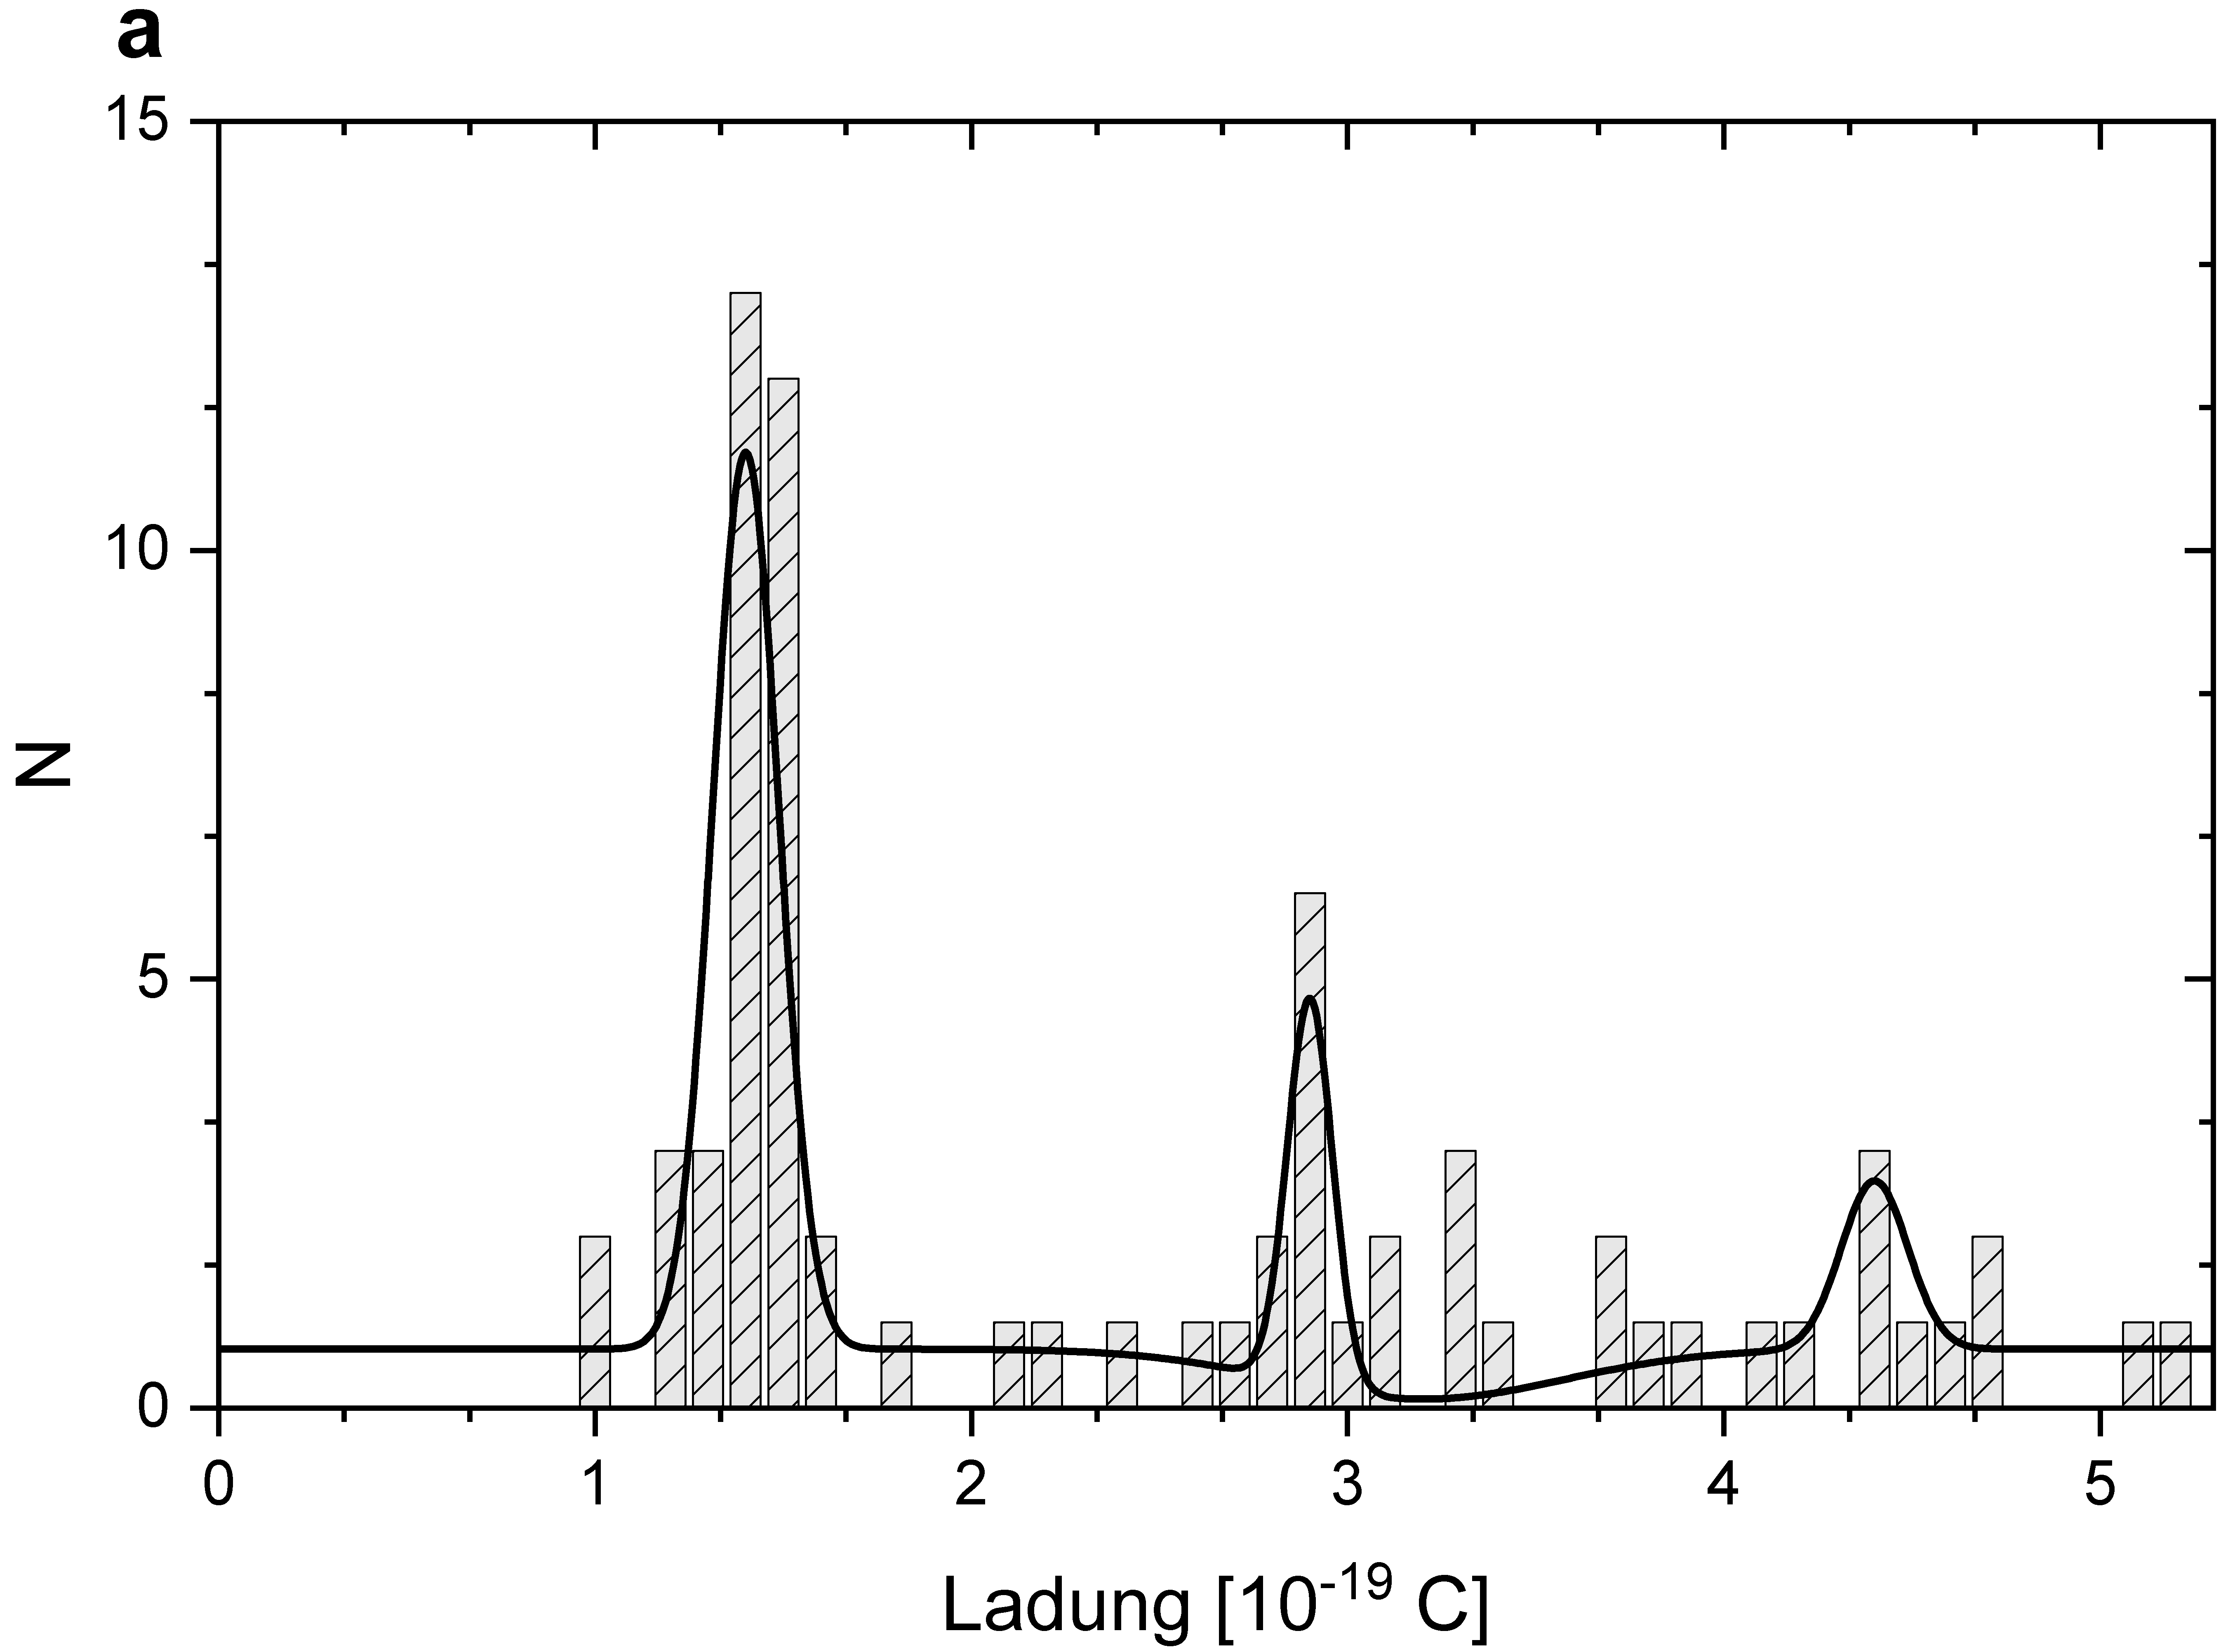
\includegraphics[width=120mm]{graphs/chargeOcc1.png}
                
                \vspace{0.3cm}
                
                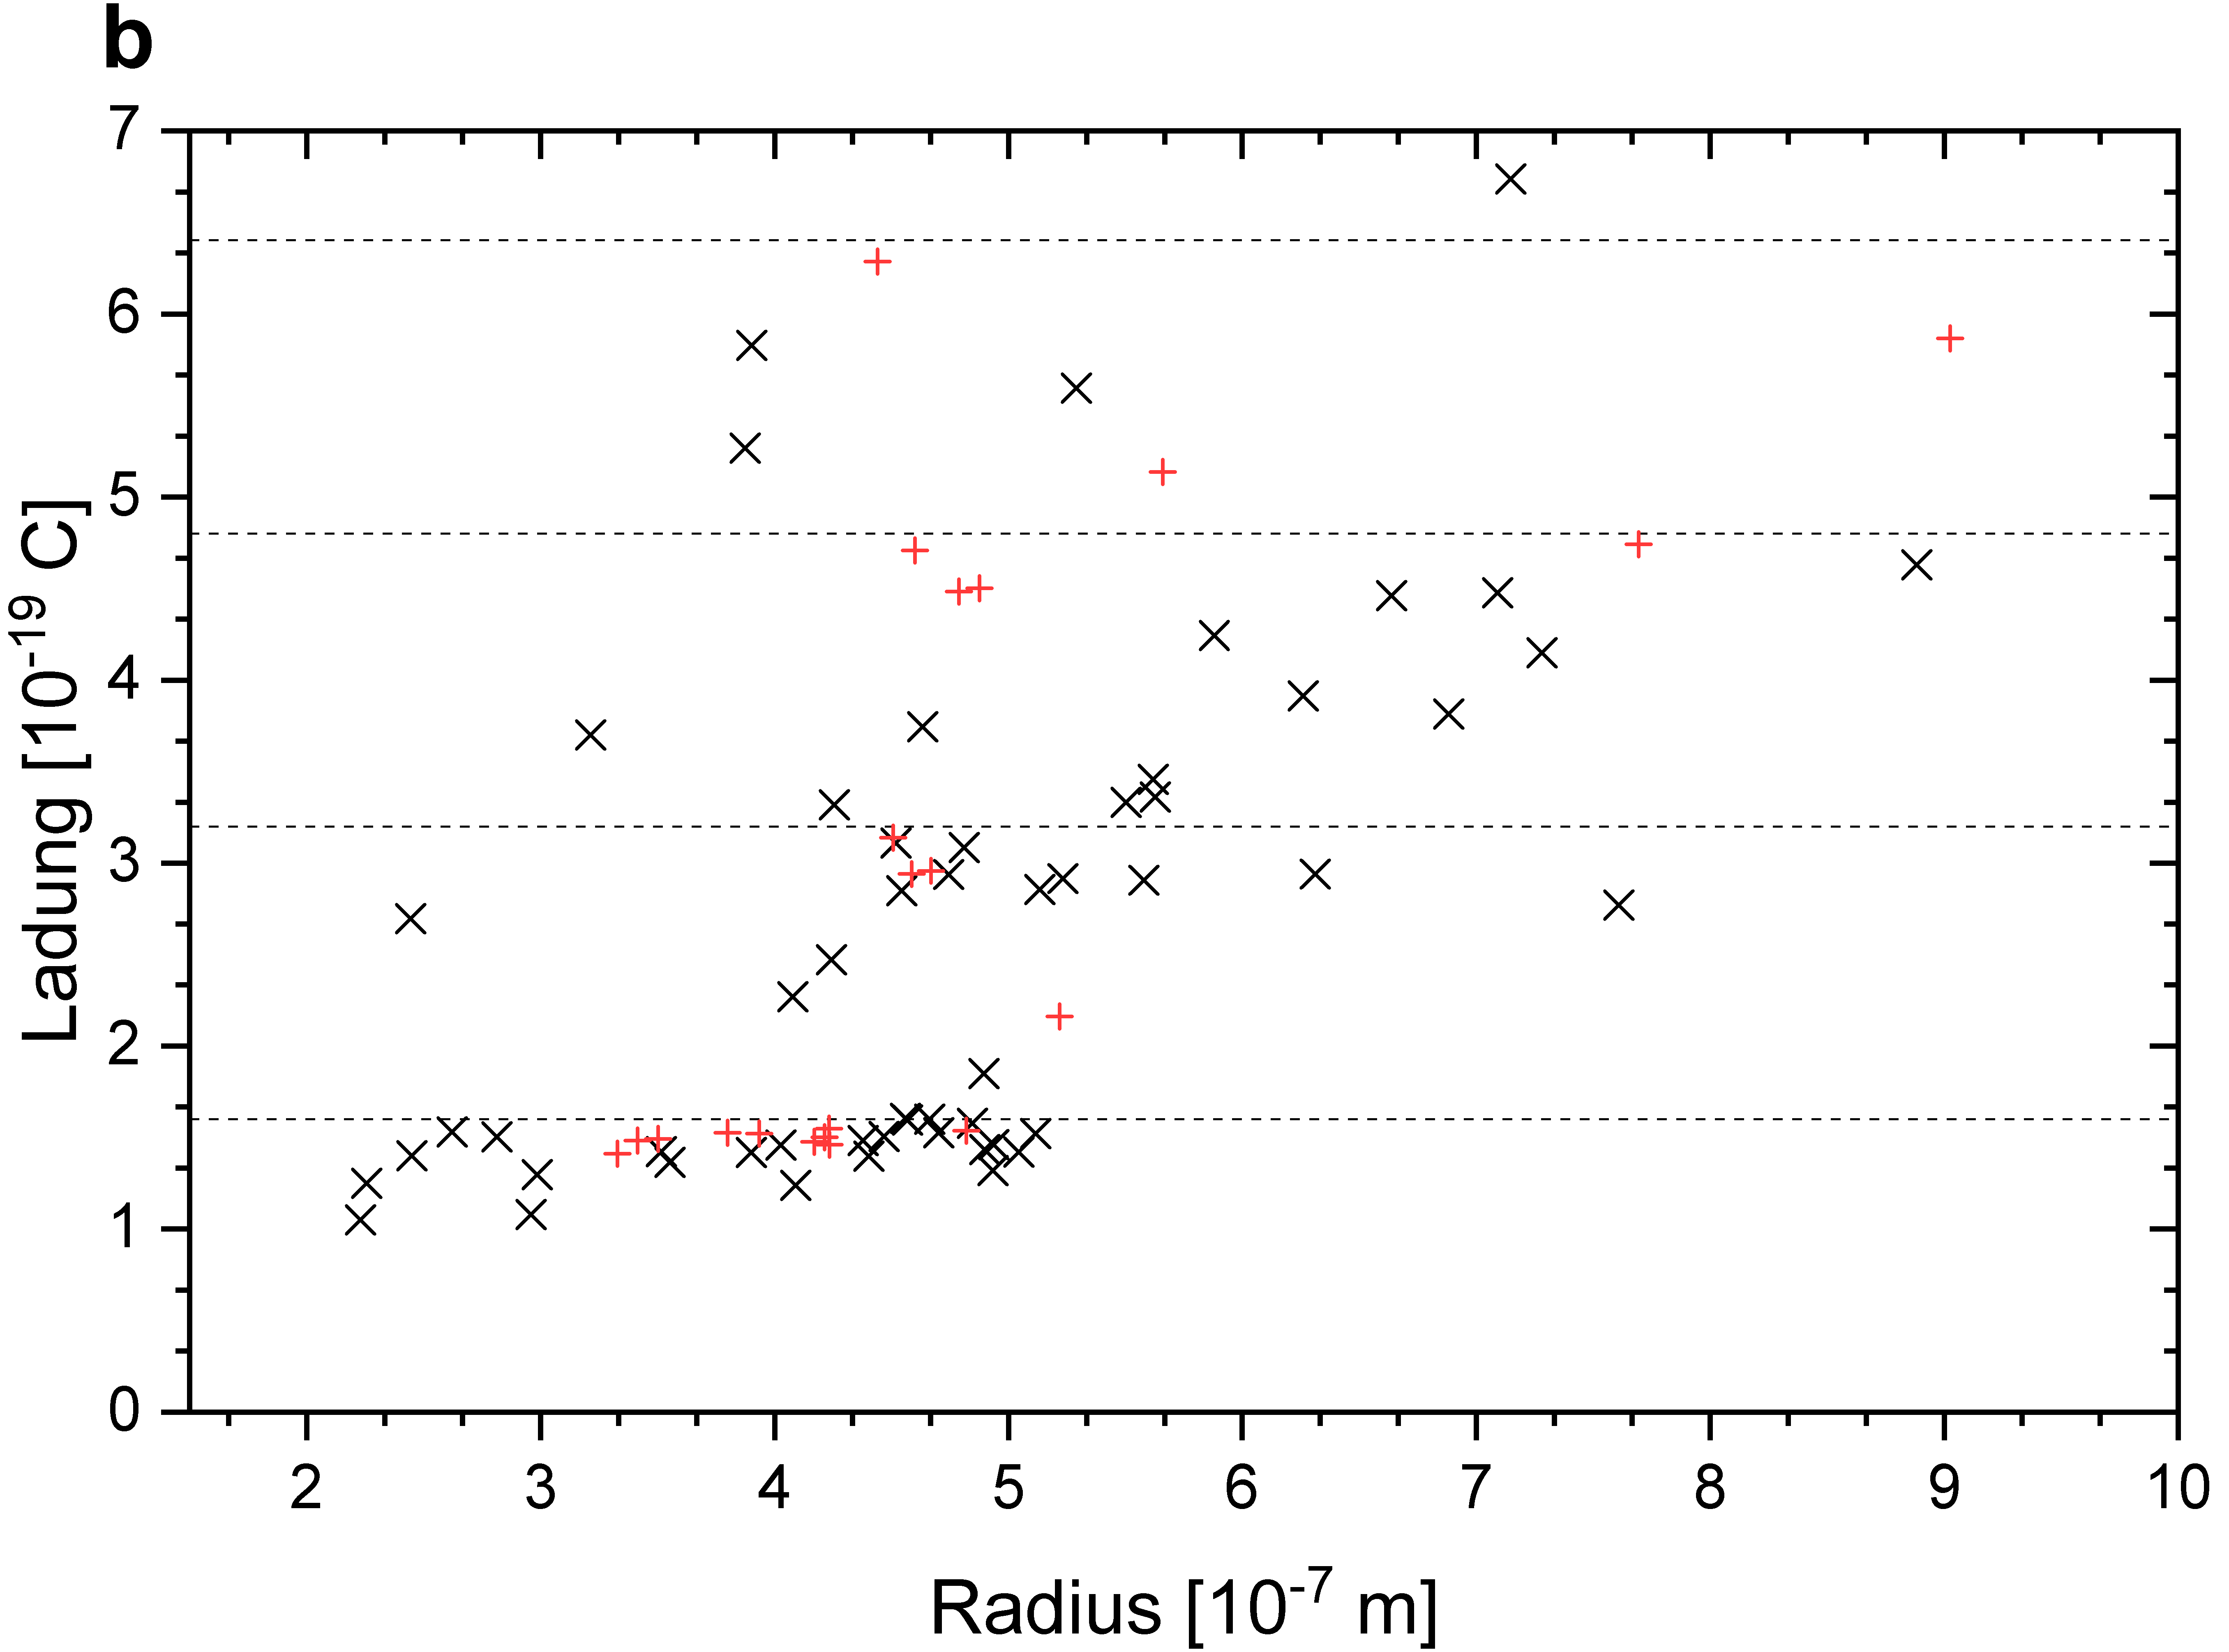
\includegraphics[width=79mm]{graphs/chargeToRad1Clean.png}
                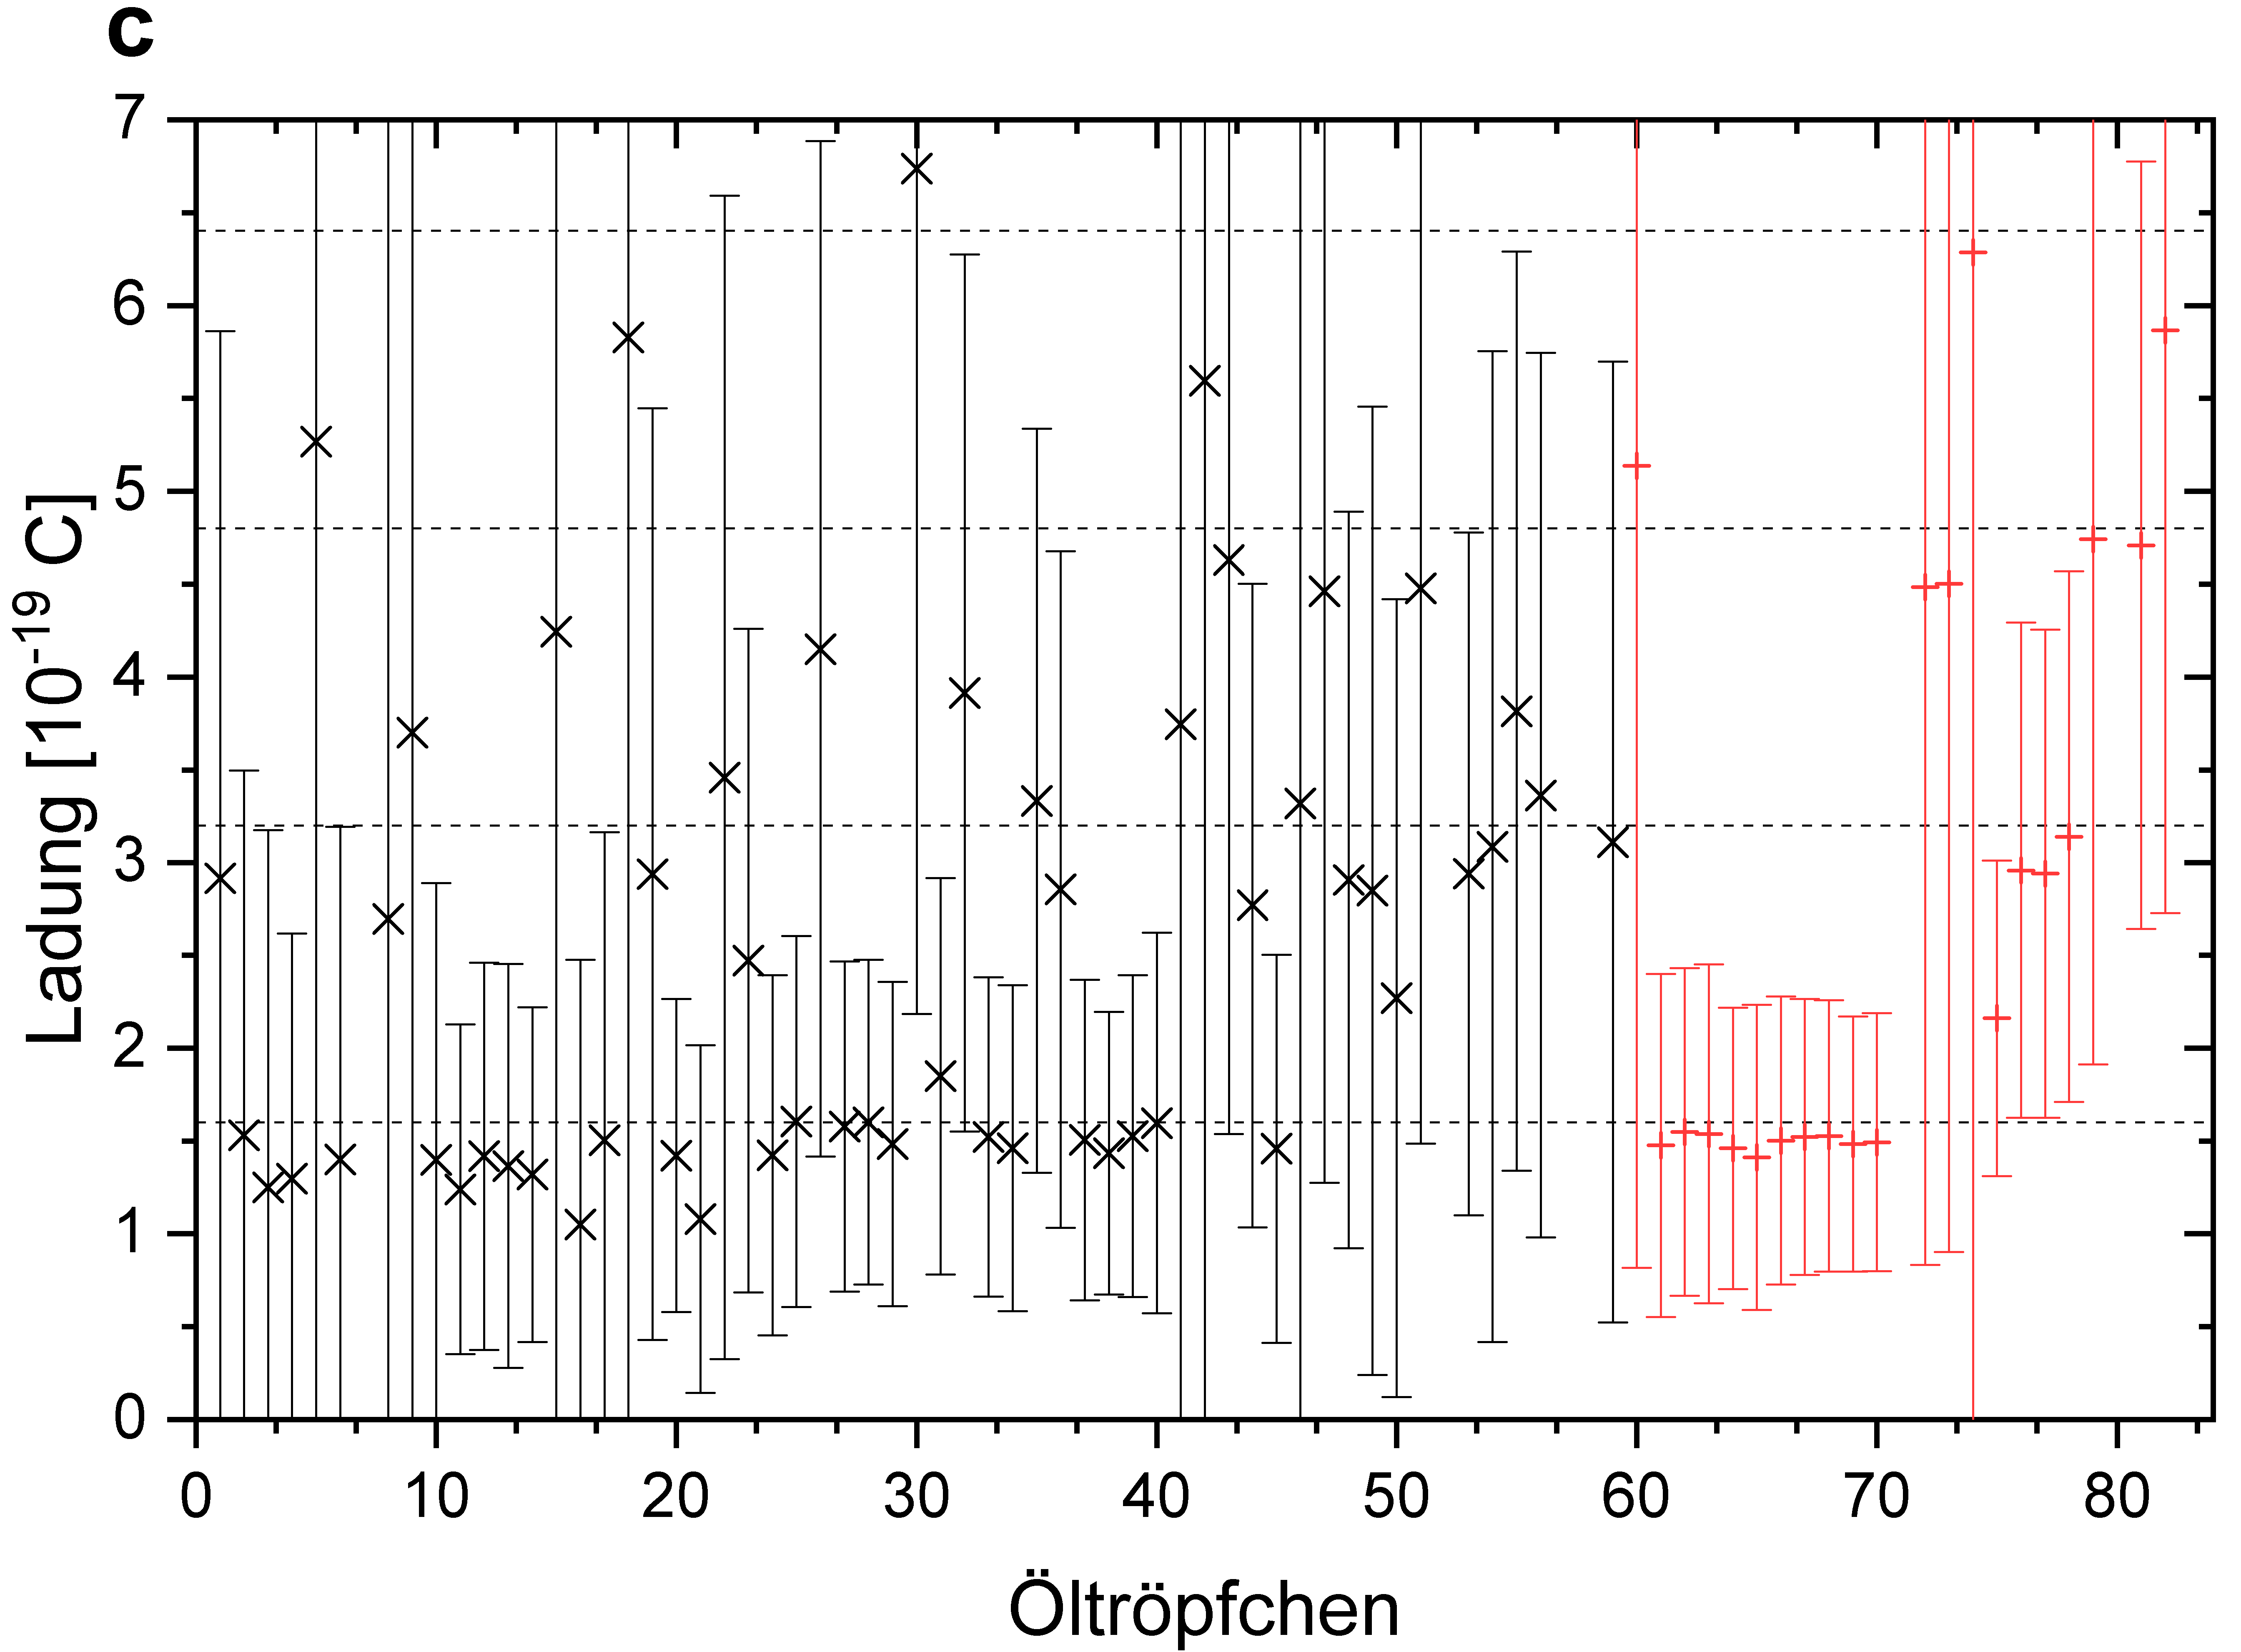
\includegraphics[width=79mm]{graphs/chargeToRadNum.png}
                \caption{\textbf{a} Erkennbare Ladungsquantisierung der einzelnen Öltröpchen. Gut erkennbar sind die drei Ausschläge, erkennbar durch die drei verbundenen Gauß-Kurven, bei vielfachen der Elementarladung. Man bemerke, dass alle Ausschläge eine Linksverschiebung von $0.1 e$ aufweisen. Bei $N$ handelt es sich um die Anzahl an Öltöpchen.
                \textbf{b} Erneute erkennbare Ladungsquantisierung. In der Nähe von $e$ befinden sich vor allem Datenpunkte der Versuchsleitung mit kleinem Fehler. Datenpunkte mit höherer Ladung weisen einen größeren Fehler auf. 
                \textbf{c} Ladung der einzelnen Öltröpchen mit Fehlerbalken. Öltröpchen mit einer Ladung größer als $7e$ sind nicht sichtbar. Gut erkennbar ist die Qualität der Datenpunkte der verschiedenen Datensätze. Datenpunkte von Datensatz 4 besitzen $t_{\mathrm{sink}}$ und $t_{\mathrm{steig}}$ im Bereich von $\sim$ 8s und weisen deshalb einen großen Fehler auf und befinden sich nicht in der Nähe von Ladung $e$.\\
                Datenpunkte der Versuchsleitung sind durch rote Pluszeichen hervorgehoben. Diese stellen eine Baseline dar.}
                \label{fig:cToRad}
            \end{figure*}
            
            \noindent Trotz des zu niedrigen Wertes für $e$ ist die Ladungsquantelung in Grafik \ref{fig:cToRad} sehr sichtbar. Für die Fehlerbalken wurde bei der Student-t-Verteilung das 68,3\% Vertrauensniveau verwendet.  
           
            
            
        \subsection{Elektronenmasse}\label{subsec:emass}
             Aus den Ergebnissen von Kapitel \ref{subsec:specelectron} und Kapitel \ref{subsec:resmilikan} lässt sich nun unter Verwendung von Formel \ref{eq:slmass} die Masse des Elektrons bestimmen. Verwendet man hierfür $\frac{e}{m} = -(1,72 \pm 0,05) \cdot 10^{11} \frac{\mathrm{C}}{\mathrm{kg}}$ und $e = -(1,43 \pm 0,63) \cdot 10^{-19}$ C, so ergibt sich
             \begin{center}
                 $\mathbf{m = (8,36 \pm 3,75) \cdot 10^{-31}}$ \textbf{kg}.
             \end{center}
             Dabei handelt es sich, aufgrund der ungenauen Elementarladung, um eine Abweichung von $\sim8,92$\% bezüglich dem Literaturwert von $m = 9,10 \cdot 10^{-31}$ kg (\cite{demtroder}). Verwendet man den Literaturwert $e = -1,60 \cdot 10^{-19}$ C, so ergibt dies
             \begin{center}
                $\mathbf{m = (9,31 \pm 0,13) \cdot 10^{-31}}$ \textbf{kg}.
             \end{center}
            Es folgt eine Abweichung von $\sim2.19$\%.
             
            
            
            
    \section{Diskussion}\label{sec:discussion}
        \subsection{Spezifische Elektronenladung}
            Der ermittelte Wert enthält den Literaturwert. Nun kann man diskutieren, wie das Experiment gestalten werden kann, damit es noch genauere Werte liefert. Zum einen sollten mehr Messdaten ermittelt werden. Die Student-t-Verteilung ist eine gute Näherung bei wenigen Messdaten, ist aber nicht mit der Genauigkeit von mehreren Messdaten zu vergleichen. Zum anderen kann eine genauere Messskala der Radien zu einem verbesserten Ergebnis führen. 
            
            \subsubsection{Erdmagnetfeld}
                Der Betrag des Erdmagnetfeldes in Fürstenfeldbruck\footnote{\url{https://www.geophysik.uni-muenchen.de/observatory/geomagnetism/taegliche-magnetogramme}, zuletzt besucht am 16.08.2019} beträgt $4,8451 \cdot 10^{-5}$ T. Berechnet man nun die minimale Magnetfeldstärke, die auf den Elektronenstrahl wirkt, beträgt diese $1,01 \cdot 10^{-3}$ T bei einem konstanten Strom von $1,3$ A. Setzt man diese beiden Werte nun ins Verhältnis, kommt man auf etwa 4,8\%. Die relative Unsicherheit der Messung beträgt 2,9\%.
                Das Erdmagnetfeld sollte also berücksichtigt werden.\\
                Eine Möglichkeit diesen Effekt nachzuweisen wäre, die Versuchsanordnung in verschiedene Himmelsrichtungen zu drehen und zu kippen. Je nach Ausrichtung und Kippwinkel sollte man eine andere Ablenkung messen können. Den Effekt im Praktikum verwendeten Versuchsaufbau zu messen, wäre nicht unbedingt möglich gewesen. Den Versuchsaufbau hätte man zwar nach verschiedenen Himmelsrichtungen ausrichten können, aber nicht kippen. Das Kippen verursacht aber eine größere Auslenkung, da der Versuchsaufbau dann so positioniert werden kann, dass das Erdmagnetfeld senkrecht auf der Geschwindigkeit der Elektronen steht. Das Magnetfeld der Helmholtzspulen steht ebenfalls senkrecht auf der Geschwindigkeit der Elektronen. Bei der selben Richtung der Magnetfelder addieren sich die Beträge. \\
                Wird der Versuchsaufbau so ausgerichtet, dass das Erdmagnetfeld maximal wirkt, kann man mit Hilfe von Formel \ref{eq:sl} Abweichungen von bis zu $\Delta r = \pm 1,7$ mm erwarten.\\
                Dieser Wert ist kleiner als die systematische Unsicherheit der Ablesegenauigkeit. Beim ermitteln der Unsicherheiten wurde bei der Student-t-Verteilung das $1-\alpha = 68,2$\% Vertrauensniveau verwendet. Hätte man einen größeres Konfidenzintervall gewählt, wäre die relative Unsicherheit wahrscheinlich größer als das Verhältnis zwischen Erdmagnetfeld und erzeugtem Magnetfeld. Die Unsicherheit würde dann die Abweichung beinhalten.

                
        \subsection{Milikanversuch} \label{subsec:dissmilikan}
             Aufgrund weniger Messdaten und einiger sowohl falschen als auch ungenauen Werten, konnte die Elementarladung nur ungenau bestimmt werden. Zudem wurden einige Messdaten nicht verwendet, da diese lediglich statistische Ungenauigkeiten hinzufügten. Trotz dessen, konnte sowohl die Ladungsquantelung als auch die Elementarladung bestimmt werden. Wie in Grafik \ref{fig:cToRad} dargestellt, ist die genannte Ladungsquantelung sichtbar, jedoch besitzen die einzelnen Werte bereits bei bei dem 68,3\% Vertrauensniveau der Studentfunktion einen großen Fehler. 
             
             \noindent Bei den Unsicherheiten geht vor allem die Ungenauigkeit im Abstand der Linien ein. Eine weitere signifikante Rolle spielt die gemessene Zeit. Aufgrund der angegebenen Reaktionszeit von $\sim0,2$ s bieten sich hierbei Öltröpfchen mit verschiedensten Fall- und Steigezeiten an, wobei diese eine Dauer von $\sim 6$ s nicht unterschreiten sollten.
             
             \noindent Wie in Grafik \ref{fig:cToRad} sichtbar, besitzen die einzelnen Datenpunkte eine relative hohe Unsicherheit. Dies kann daraus folgen, dass eine nicht bekannte Fehlerquelle nicht einbezogen wurde. Trotz dessen, stimmen die berechneten Unsicherheiten gut mit der abweichenden Bestimmung der Elementarladung zusammen.\\
             Aufgrund der kurzen $t_{\mathrm{steig}}$ und $t_{\mathrm{sink}}$ wird dieser hier besonders hervorgehoben. Bei diesem Datensatz handelt es sich um diesen, der die größte Unsicherheit aufweist. Wie bereits angemerkt, folgt dies aus großen Ladung der gemessenen Öltröpfchen. Eine genaue Analyse dieses Datensatz lieferte hierbei zudem Öltröpfchen mit dem größten Radius. Dies erklärt die große Ladung und kurze $t_{\mathrm{steig}}$ und $t_{\mathrm{sink}}$ dieser Öltröpfchen. Eine Darstellung findet sich in Abbildung \ref{fig:cToRad}c .
             Bei der Ermittelung der Unsicherheiten wurden Schwankungen der Temperatur und des Druckes nicht berücksichtigt, da diese viel kleiner sind als die anderen angenommen Unsicherheiten. Damit das Ergebnis sich signifikant ändert müssen große Schwankungen stattgefunden haben. Da wir uns aber sicher sein können, dass sich an diesem Tag die Temperatur nicht um $\pm 5$ °C und der Druck nicht um $\pm 60$ mb verändert hat, können wir eine maximale Unsicherheit von höchstens 1\% ausgehen. Dementsprechend haben wir die Annahme getroffen, dass die anderen Unsicherheiten diese geringe Schwankung schon beinhalten.
             
             
         \subsection{Elektronenmasse}
            Eine genaue Bestimmung der Elektronenmasse setzt eine genaue bestimmen der spezifischen Elektronenladung $e/m$ und der Elementarladung voraus. Wie in Kapitel \ref{subsec:emass} aufgeführt, haben bereits kleine Ungenauigkeiten und Unsicherheiten große Auswirkungen auf das Resultat der dadurch berechnete Elektronenmasse. Trotz der ungenauen Berechnung der Elektronenladung, war es möglich einen Näherungsweise korrekten Wert der Elektronenmasse zu berechnen.
            
            \noindent Aufgrund der verschiedenen Unsicherheiten, sowohl statistischer als auch systematischer Natur, sind für eine genaue Berechnung der Elementarladung deutlich mehr Messwerte nötig. Dies ist vor allem in der Standardabweichung des Mittelwerts der einzelnen Parameter in Gleichung \ref{eq:radius} und Gleichung \ref{eq:charge} erkennbar. 
       
       
    \section{Zusammenfassung}
        Zusammenfassend lässt sich erkennen, dass das Modell zur Ermittlung der spezifischen Elektronenladung einen einfachen Aufbau hat und genaue Ergebnisse, trotz weniger Messdaten,  liefert.\\
        Die Auswertung der Daten des Milikanversuchs erwies sich als sehr schwierig. Zwar konnte die zu erwartende Ladungsquantelung veranschaulicht werden, aber mit einer viel zu hohen Unsicherheit. Die möglichen Fehlerquellen wurden in Kapitel \ref{subsec:dissmilikan} aufgeführt. Der Milikanversuch ist im Allgemeinen ein sehr aufwendiges Experiment, dass eine Vielzahl an Messdaten zur korrekten Auswertung benötigt. Hinzu kommt, dass die Ermittlung der Daten nur teilweise automatisierbar ist, weswegen es ein sehr zeitaufwendiger Versuch ist. 
            
        
        
    % References
    \bibliographystyle{mnras}
    \bibliography{Ausarbeitung.bib}
    


    % Appendix
    %\newpage
    \appendix
    \section{Fehlerrechnung}
        \subsection{Spezifische Elektronenladung}
            Für die statistische Unsicherheit wurde zuerst der Mittelwert der Messergebnisse gebildet. Es folgte die Berechnung der Standardabweichung und der Mittelwert der Standardabweichung. Aufgrund weniger Messergebnisse wurde eine Korrektur mittels Student-t-Verteilung vorgenommen. Das verwendete Vertrauensniveau beträgt $68,2\%$. Anschließend wurden die Unsicherheiten mittels partieller Differentiation fortgepflanzt.\\
            Die systematischen Unsicherheiten wurden mittels linearer Addition fortgepflanzt. Die Begründung der Wahl der Werte befindet sich in Kapitel \ref{subsec:specelectron}.\\
            Mittels linearer Addition wurden die Werte der Unsicherheiten verknüpft. Da die Messwerte die selbe Genauigkeit aufweisen, können die sechs Einzelwerte mittels des gewichteten Mittelwerts zu einem Wert verknüpft werden. 
    
        \subsection{Milikanversuch}
            Für die Berechnung der Unsicherheiten der einzelnen Punkte wurden die Unsicherheiten von Fallstrecke, Fallzeit, Plattenabstand, Reaktionszeit und Spannungsmessgerät mit einbezogen.
            
            \noindent Man bilde für jeden Datenpunkt eine Unsicherheit bestehend aus der Kombination aller bekannten Fehlerquellen. Diese Unsicherheiten sind in Grafik \ref{fig:cToRad} dargestellt. Dabei wurde $\overline{\Delta} U = 1$ V, $\overline{\Delta} d = 0,05$ mm, $\overline{\Delta} s_{\mathrm{steig}} = \overline{\Delta} s_{\mathrm{sink}} = 0,05$ mm, $\overline{\Delta} t_{\mathrm{steig}} = \overline{\Delta} t_{\mathrm{sink}} = 0,2$ s gewählt. Die Unsicherheit wurden mittels linearer Addition fortgepflanzt\footnotemark[1].
                
            
        \subsection{Elektronenmasse}
            Aufgrund der statistischen Unabhängigkeit der Berechnungen von spezifischer Ladung und der Elementarladung, kann der eingehende Fehler in die berechnete Masse wie folgt berechnet werden.
            \begin{equation}
                \Delta \overline{m} = \Delta \overline{e} \left[\frac{\partial m}{\partial e}\right] + \Delta \overline{e}_{\mathrm{spezifisch}} \left[\frac{\partial m}{e_{\mathrm{spezifisch}}}\right]  = \pm 3,75 \cdot 10^{-31}
            \end{equation}
            Hierbei handelt es sich um die Fehlerfortplanzung der spezifischer Ladung und Elementarladung mittels partieller Ableitung.
    
    % Don't change these lines
    \label{lastpage}
\end{document}
